\documentclass[12pt]{article}
\usepackage{amsmath, amssymb}
\usepackage{graphicx}
\usepackage{enumerate}
\usepackage{natbib}
\usepackage{float}
\usepackage{subfig}
\usepackage{pdfpages}
\renewcommand{\tablename}{Supplementary Table}
\renewcommand{\figurename}{Supplementary Figure}
\usepackage{url} % not crucial - just used below for the URL 

%\pdfminorversion=4
% NOTE: To produce blinded version, replace "0" with "1" below.
\newcommand{\blind}{1}

% DON'T change margins - should be 1 inch all around.
\addtolength{\oddsidemargin}{-.5in}%
\addtolength{\evensidemargin}{-1in}%
\addtolength{\textwidth}{1in}%
\addtolength{\textheight}{1.7in}%
\addtolength{\topmargin}{-1in}%




\begin{document}

\bibliographystyle{agsm}

\def\spacingset#1{\renewcommand{\baselinestretch}%
{#1}\small\normalsize} \spacingset{1}


%%%%%%%%%%%%%%%%%%%%%%%%%%%%%%%%%%%%%%%%%%%%%%%%%%%%%%%%%%%%%%%%%%%%%%%%%%%%%%

\if1\blind
{
  \title{\bf Supplementary Materials for \textit{Dynamic Prediction of Milestones for Survival Endpoints in Metastatic Solid Tumor Cancer Clinical Trials}}
  \author{Sidi Wang\\
    Department of Biostatistics, University of Michigan\\
    Kelley M Kidwell \\
    Department of Biostatistics, University of Michigan\\
    Bo Huang \\
    Pfizer Inc., New York, NY, U.S.A. \\
    and \\
    Satrajit Roychoudhury \\
    Pfizer Inc., New York, NY, U.S.A.}
  \maketitle
} \fi

\if0\blind
{
  \bigskip
  \bigskip
  \bigskip
  \begin{center}
    {\LARGE\bf Improving prediction of overall survival using joint modeling for oncology studies with solid tumor response}
\end{center}
  \medskip
} \fi

\bigskip


\noindent%

\vfill


\spacingset{1.9} % DON'T change the spacing!
\newpage
\begin{figure}[H]
    \centering
    \subfloat[]{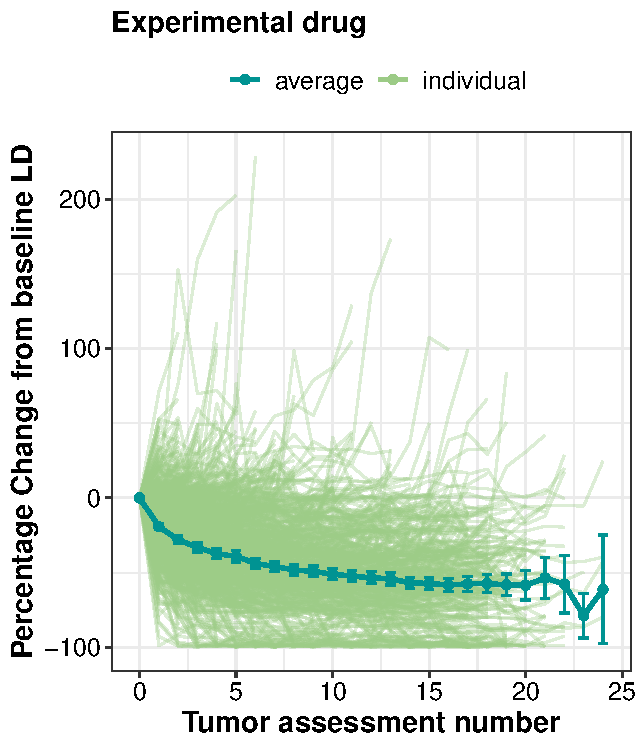
\includegraphics[width=0.45\textwidth]{img/profile_LD_exp.pdf}\label{fig:profile_LD_exp}}
    \hfill
    \subfloat[]{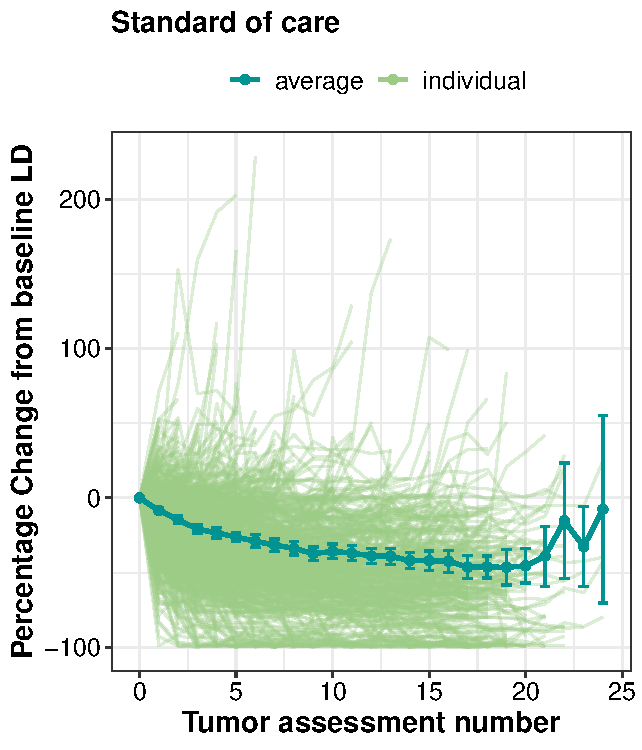
\includegraphics[width=0.45\textwidth]{img/profile_LD_soc.pdf}\label{fig:profile_LD_soc}}
    \caption{Profile plot of the sum of the longest diameter of target lesions}
    \label{fig:profile_LD}
\end{figure}

\newpage
\begin{figure}[H]
    \centering
    \subfloat[]{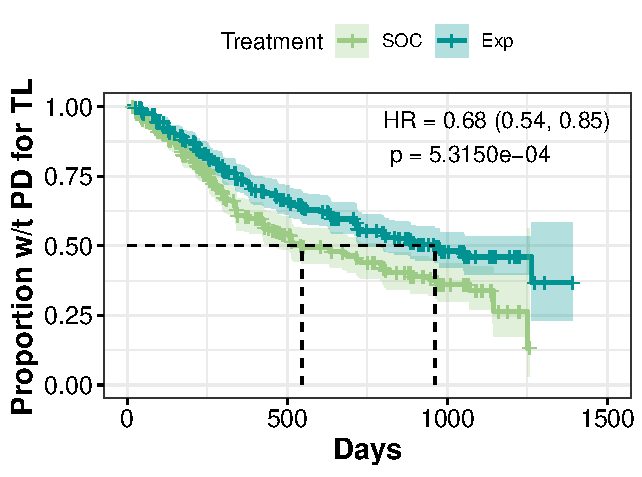
\includegraphics[width=0.45\textwidth]{img/TL_KMplot.pdf}\label{fig:TL_KMplot}}
    \subfloat[]{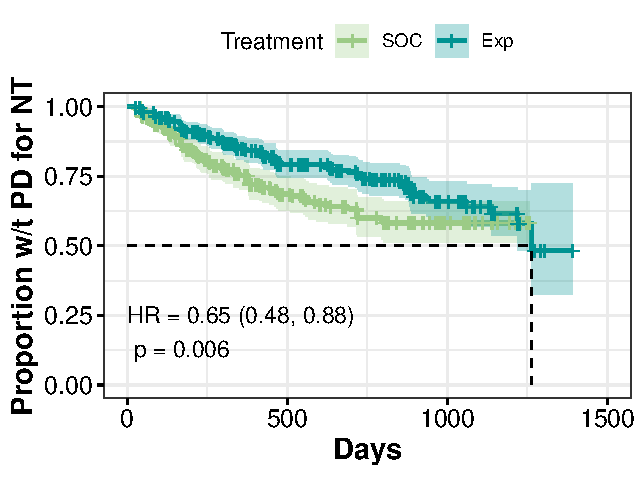
\includegraphics[width=0.45\textwidth]{img/NT_KMplot.pdf}\label{fig:NT_KMplot}}
    \hfill
    \subfloat[]{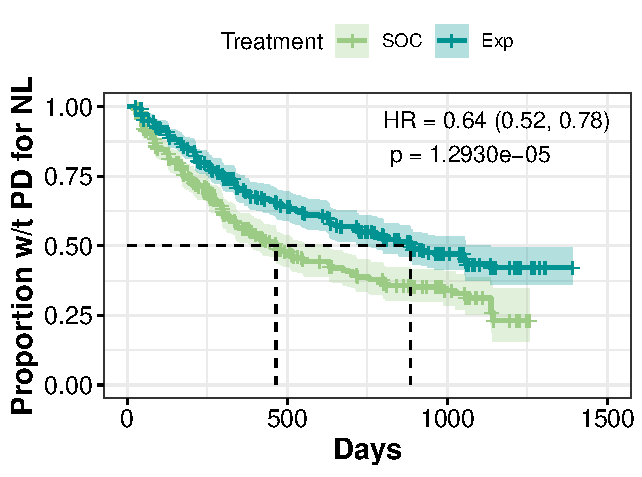
\includegraphics[width=0.45\textwidth]{img/NL_KMplot.pdf}\label{fig:NL_KMplot}}
    \subfloat[]{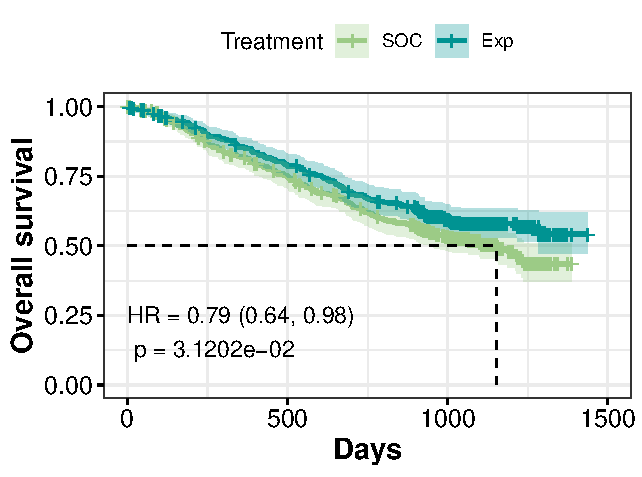
\includegraphics[width=0.45\textwidth]{img/OS_KMplot.pdf}\label{fig:OS_KMplot}}
    \hfill
    \subfloat[]{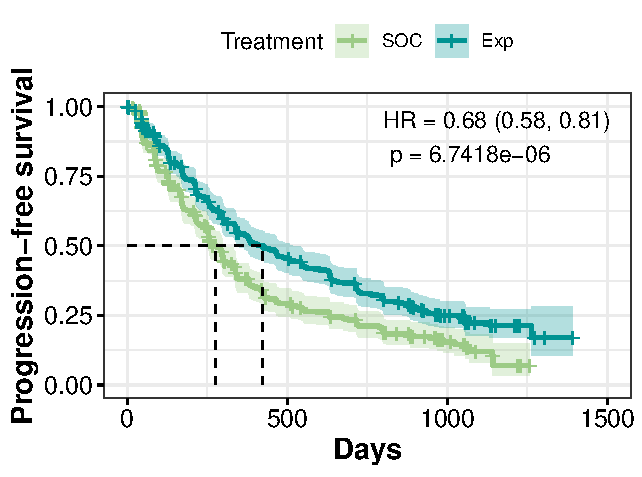
\includegraphics[width=0.45\textwidth]{img/PFS_KMplot.pdf}\label{fig:PFS_KMplot}}
    \caption{Kaplan-Meier plots at the time of updated OS analysis considering target lesions progressive disease (PD) (a), non-target lesions PD (b), new lesions PD (c), overall survival (d), and progression-free survival (e).}
\end{figure}

%\newpage
%\begin{figure}[H]
%    \centering
%    \subfloat[]{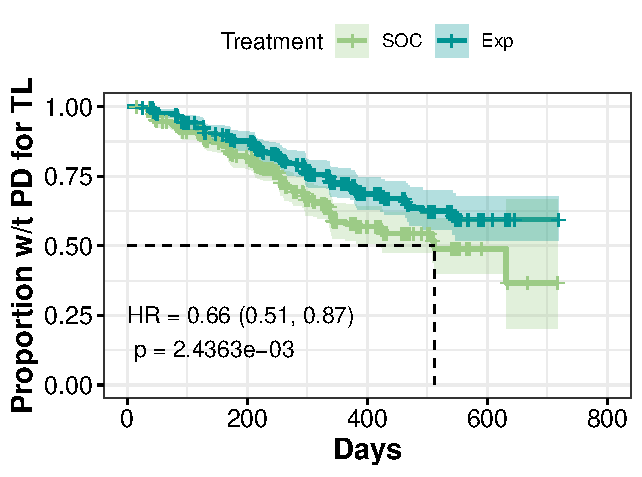
\includegraphics[width=0.40\textwidth]{img/TL_KMplot_PA.pdf}\label{fig:TL_KMplot_PA}}
%    \subfloat[]{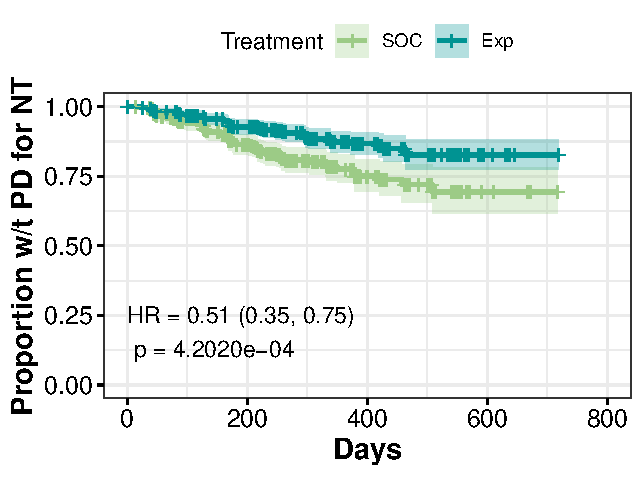
\includegraphics[width=0.40\textwidth]{img/NT_KMplot_PA.pdf}\label{fig:NT_KMplot_PA}}
%    \hfill
%    \subfloat[]{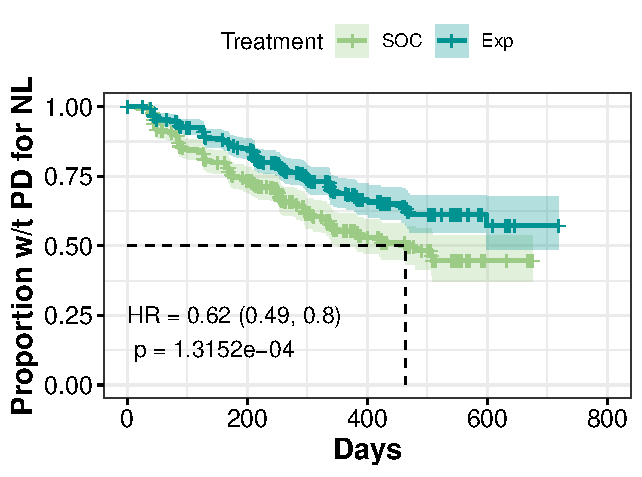
\includegraphics[width=0.40\textwidth]{img/NL_KMplot_PA.pdf}\label{fig:NL_KMplot_PA}}
%    \subfloat[]{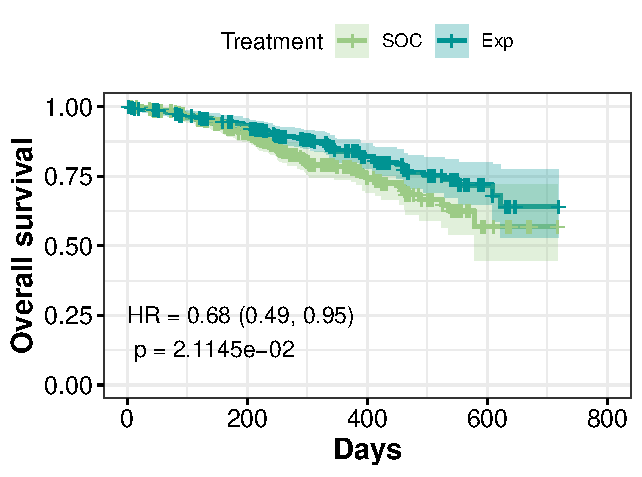
\includegraphics[width=0.40\textwidth]{img/OS_KMplot_PA.pdf}\label{fig:OS_KMplot_PA}}
%    \hfill
%    \subfloat[]{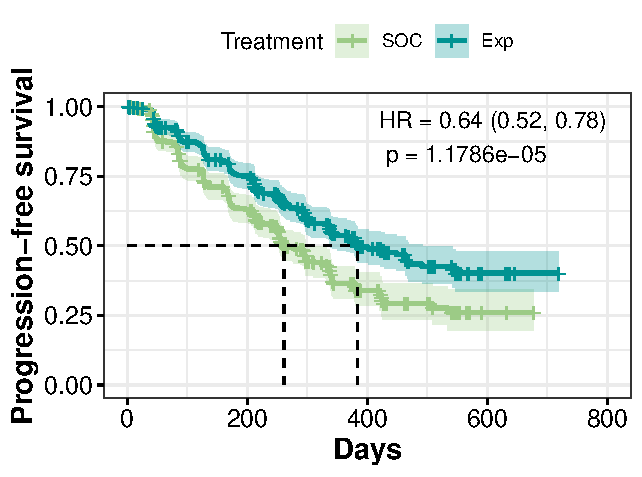
\includegraphics[width=0.40\textwidth]{img/PFS_KMplot_PA.pdf}\label{fig:PFS_KMplot_PA}}
%    \caption{Kaplan-Meier plots at the time of primary analysis considering target lesions progressive disease (PD) (a), non-target lesions PD (b), new lesions PD (c), overall survival (d), and progression-free survival (e).. \label{fig:KMplot_PA}}
%\end{figure}



\newpage
\section{Likelihood derivation for the joint model between target lesion and OS}
The marginal distribution of the observed measurements $\mu$ is easily obtained. The likelihood for the observed data can be factorized as the product of this marginal distribution and the conditional distribution of OS, given the observed values of $\mu$. Let $\boldsymbol{\theta}_1$ denote the combined vector of unknown parameters. Conditional on lesion measurements $\mu$, OS is independent of these measurements $\mu$, so we can write the likelihood $L=L(\boldsymbol{\theta}_1, \mu, OS)$ as
$L=L_{\mu}(\boldsymbol{\theta}_1,\mu)  \times L_{OS| \mu}(\boldsymbol{\theta}_1,OS|\mu)
$,
where $L_{\mu}(\boldsymbol{\theta}_1,\mu)$ is of standard form corresponding to the marginal multivariate normal distribution of $\mu$ and
$$
L_{OS|\mu}(\boldsymbol{\theta}_1, OS|\mu)=\prod_i \bigg\{ \bigg[\lambda_0 (t) \exp(\textbf{Z}_i' \boldsymbol{\beta}_{\rm OS}+\lambda \mu_{i}(t)) \bigg]^{\delta_{OS,i}} 
$$
$$\times \exp \bigg[ -\int_0^{y_{OS,i}} \lambda_0(t) \exp(\textbf{Z}_i' \boldsymbol{\beta}_{\rm OS}+\lambda \mu_{i}(t))dt\bigg]\bigg\},
$$
Here, $y_{OS,i}=\min(t_{OS,i},c_{OS,i})$ and $\delta_{OS,i}=I(t_{OS,i}\leq c_{OS,i})$. $c_{OS,i}$ is the censoring time for the $i$th participant and $t_{OS,i}$ is the true event time.


\newpage
\section{Likelihood derivation for the copula model of the non-target lesion and OS}
For non-target lesion, we define $y_{\rm NT}=\mathrm{min}(t_{\rm NT}, c_{\rm NT})$ and
$\delta_{\rm NT}=I(t_{\rm NT} \le c_{\rm NT})$,
where $c_{\rm NT}$ and $I(\cdot)$ denote the censoring time and the indicator function,
respectively; and define $y_{\rm OS}$ and $\delta_{\rm OS}$ similarly for OS.

Depending on the censoring pattern, the observed data for the $i$th participant falls into one of the following mutually exclusive cases: 1) both $t_{NT}$ and $t_{OS}$ are observed ($\delta_{NT}$=1, $\delta_{OS}$=1), 2) $t_{NT}$ is observed and $t_{OS}$ is censored ($\delta_{NT}$=1, $\delta_{OS}$=0), 3) $t_{NT}$ is censored and $t_{OS}$ is observed ($\delta_{NT}$=0, $\delta_{OS}$=1), and 4) both $t_{NT}$ and $t_{OS}$ are censored ($\delta_{NT}$=0, $\delta_{OS}$=0). Based on these four scenarios, we derive the likelihood of the copula model. 

Let
$\boldsymbol{\theta}_2=(\boldsymbol{\beta_{\rm NT}}, \alpha_{\rm NT}, \lambda_{\rm NT}, \boldsymbol{\beta_{\rm OSNT}},
\alpha_{\rm OSNT}, \lambda_{\rm OS}, \eta_{\rm NT})$,  then the
likelihood for the $i$th patient with ${\rm Data}_i=(y_{\rm NT}, y_{\rm OS},
\delta_{\rm NT}, \delta_{\rm OS}, \textbf{Z})_i$ is given by
$$
L(\boldsymbol{\theta}_2|{\rm Data}_i)
=L_1^{\delta_{\rm NT}\delta_{\rm OS}}
L_2^{\delta_{\rm NT}(1-\delta_{\rm OS})}L_3^{(1-\delta_{\rm NT})\delta_{\rm OS}}
L_4^{(1-\delta_{\rm NT})(1-\delta_{\rm OS})}, 
$$

where
$$
L_1=\frac{\partial^2\, S_1(t_{\rm NT}, t_{\rm OS}|\textbf{Z})}{\partial t_{\rm NT} \partial t_{\rm OS}}\big|_{t_{\rm NT}=y_{\rm NT},t_{\rm OS}=y_{\rm OS}}
$$
$$
=\bigg(\eta_{\rm NT}+1\bigg)\bigg(\mathrm{exp}\{-\gamma_{\rm NT} y_{\rm NT}^{\alpha_{\rm NT}}
\mathrm{exp}(\textbf{Z}' \boldsymbol{\beta_{\rm NT}} )\} \mathrm{exp}\{-\gamma_{\rm OS} y_{\rm OS}^{\alpha_{\rm OSNT}}
\mathrm{exp}(\textbf{Z}' \boldsymbol{\beta_{\rm OSNT}} )\}\bigg)^{-(\eta_{\rm NT}+1)}
$$
$$
\times \bigg(\mathrm{exp}\{-\gamma_{\rm NT} y_{\rm NT}^{\alpha_{\rm NT}}
\mathrm{exp}(\textbf{Z}' \boldsymbol{\beta_{\rm NT}} )\}^{-\eta_{\rm NT}}+\mathrm{exp}\{-\gamma_{\rm OS} y_{\rm OS}^{\alpha_{\rm OSNT}}
\mathrm{exp}(\textbf{Z}' \boldsymbol{\beta_{\rm OSNT}} )\}^{-\eta_{\rm NT}}-1\bigg)^{-\frac{2\eta_{\rm NT}+1}{\eta_{\rm NT}}}
$$
$$
\times \gamma_{\rm NT} \alpha_{\rm NT} y_{\rm NT}^{{\alpha_{\rm NT} -1}} \exp(\textbf{Z}' \boldsymbol{\beta_{\rm NT}}) \mathrm{exp}\{-\gamma_{\rm NT} t^{\alpha_{\rm NT}}
\mathrm{exp}(\textbf{Z}' \boldsymbol{\beta_{\rm NT}} )\}
$$
$$
\times \gamma_{\rm OS} \alpha_{\rm OSNT} y_{\rm OS}^{{\alpha_{\rm OSNT} -1}} \exp(\textbf{Z}' \boldsymbol{\beta_{\rm OSNT}}) \mathrm{exp}\{-\gamma_{\rm OS} t^{\alpha_{\rm OSNT}}
\mathrm{exp}(\textbf{Z}' \boldsymbol{\beta_{\rm OSNT}} )\}
$$

and

$$
L_2=-\frac{\partial S_1(t_{\rm NT}, t_{\rm OS}|\textbf{Z})}{\partial t_{\rm NT}}\bigg|_{t_{\rm NT}=y_{\rm NT},t_{\rm OS}=y_{\rm OS}}
$$
$$
=-\bigg(\mathrm{exp}\{-\gamma_{\rm NT} y_{\rm NT}^{\alpha_{\rm NT}}
\mathrm{exp}(\textbf{Z}' \boldsymbol{\beta_{\rm NT}} )\}\bigg)^{-(\eta_{\rm NT}+1)}
$$
$$
\times \bigg(\mathrm{exp}\{-\gamma_{\rm NT} y_{\rm NT}^{\alpha_{\rm NT}}
\mathrm{exp}(\textbf{Z}' \boldsymbol{\beta_{\rm NT}} )\}^{-\eta_{\rm NT}}+\mathrm{exp}\{-\gamma_{\rm OS} y_{\rm OS}^{\alpha_{\rm OSNT}}
\mathrm{exp}(\textbf{Z}' \boldsymbol{\beta_{\rm OSNT}} )\}^{-\eta_{\rm NT}}-1\bigg)^{-\frac{\eta_{\rm NT}+1}{\eta_{\rm NT}}}
$$
$$
\times \gamma_{\rm NT} \alpha_{\rm NT} y_{\rm NT}^{{\alpha_{\rm NT} -1}} \exp(\textbf{Z}' \boldsymbol{\beta_{\rm NT}}) \mathrm{exp}\{-\gamma_{\rm NT} t^{\alpha_{\rm NT}}
\mathrm{exp}(\textbf{Z}' \boldsymbol{\beta_{\rm NT}} )\}
$$

and

$$
L_3=-\frac{\partial S_1(t_{\rm NT}, t_{\rm OS}|\textbf{Z})}{\partial t_{\rm OS}}\bigg|_{t_{\rm NT}=y_{\rm NT},t_{\rm OS}=y_{\rm OS}}
$$
$$
=-\bigg(\mathrm{exp}\{-\gamma_{\rm OS} y_{\rm OS}^{\alpha_{\rm OSNT}}
\mathrm{exp}(\textbf{Z}' \boldsymbol{\beta_{\rm OSNT}} )\}\bigg)^{-(\eta_{\rm NT}+1)}
$$
$$
\times \bigg(\mathrm{exp}\{-\gamma_{\rm NT} y_{\rm NT}^{\alpha_{\rm NT}}
\mathrm{exp}(\textbf{Z}' \boldsymbol{\beta_{\rm NT}} )\}^{-\eta_{\rm NT}}+\mathrm{exp}\{-\gamma_{\rm OS} y_{\rm OS}^{\alpha_{\rm OSNT}}
\mathrm{exp}(\textbf{Z}' \boldsymbol{\beta_{\rm OSNT}} )\}^{-\eta_{\rm NT}}-1\bigg)^{-\frac{\eta_{\rm NT}+1}{\eta_{\rm NT}}}
$$
$$
\times \gamma_{\rm OS} \alpha_{\rm OSNT} y_{\rm OS}^{{\alpha_{\rm OSNT} -1}} \exp(\textbf{Z}' \boldsymbol{\beta_{\rm OSNT}}) \mathrm{exp}\{-\gamma_{\rm OS} t^{\alpha_{\rm OSNT}}
\mathrm{exp}(\textbf{Z}' \boldsymbol{\beta_{\rm OSNT}} )\}
$$

and

$$
L_4=S_1(t_{\rm NT}, t_{\rm OS}|\textbf{Z})\bigg|_{t_{\rm NT}=y_{\rm NT},t_{\rm OS}=y_{\rm OS}}
$$
$$
=\{\mathrm{exp}\{-\gamma_{\rm NT} y_{\rm NT}^{\alpha_{\rm NT}}
\mathrm{exp}(\textbf{Z}' \boldsymbol{\beta_{\rm NT}} )\}^{-\eta_{\rm NT}}
+\mathrm{exp}\{-\gamma_{\rm OS} y_{\rm OS}^{\alpha_{\rm OSNT}}
\mathrm{exp}(\textbf{Z}' \boldsymbol{\beta_{\rm OSNT}} )\}^{-\eta_{\rm NT}}-1\}^{-1/\eta_{\rm NT}}
$$
For a given subject, L1, L2, L3 and L4 correspond to the likelihood components that both NT and OS are observed, NT is observed but OS is censored, NT is censored but OS is observed, and both NT and OS are censored, respectively.

\newpage
\section{Likelihood derivation for the copula model of the new lesion and OS}
For new lesion, we define $y_{\rm NL}=\mathrm{min}(t_{\rm NL}, c_{\rm NL})$ and
$\delta_{\rm NL}=I(t_{\rm NL} \le c_{\rm NL})$,
where $c_{\rm NL}$ and $I(\cdot)$ denote the censoring time and the indicator function,
respectively; and define $y_{\rm OS}$ and $\delta_{\rm OS}$ similarly for OS.

Depending on the censoring pattern, the observed data for the $i$th participant falls into one of the following mutually exclusive cases: 1) both $t_{NL}$ and $t_{OS}$ are observed ($\delta_{NL}$=1, $\delta_{OS}$=1), 2) $t_{NL}$ is observed and $t_{OS}$ is censored ($\delta_{NL}$=1, $\delta_{OS}$=0), 3) $t_{NL}$ is censored and $t_{OS}$ is observed ($\delta_{NL}$=0, $\delta_{OS}$=1), and 4) both $t_{NL}$ and $t_{OS}$ are censored ($\delta_{NL}$=0, $\delta_{OS}$=0). Based on these four scenarios, we derive the likelihood of the copula model. 
Let
$\boldsymbol{\theta}_3=(\boldsymbol{\beta_{\rm NL}}, \alpha_{\rm NL}, \lambda_{\rm NL}, \boldsymbol{\beta_{\rm OSNL}},
\alpha_{\rm OSNL}, \lambda_{\rm OS}, \eta_{\rm NL})$,  then the likelihood for the $i$th patient with ${\rm Data}_i=(y_{\rm NL}, y_{\rm OS},
\delta_{\rm NL}, \delta_{\rm OS}, \textbf{Z})_i$ is given by
$$
L(\boldsymbol{\theta}_3|{\rm Data}_i)
=L_1^{\delta_{\rm NL}\delta_{\rm OS}}
L_2^{\delta_{\rm NL}(1-\delta_{\rm OS})}L_3^{(1-\delta_{\rm NL})\delta_{\rm OS}}
L_4^{(1-\delta_{\rm NL})(1-\delta_{\rm OS})}, 
$$
where
$$
L_1=\frac{\partial^2\, S_2(t_{\rm NL}, t_{\rm OS}|\textbf{Z})}{\partial t_{\rm NL} \partial t_{\rm OS}}\big|_{t_{\rm NL}=y_{\rm NL},t_{\rm OS}=y_{\rm OS}}
$$
$$
=\bigg(\eta_{\rm NL}+1\bigg)\bigg(\mathrm{exp}\{-\gamma_{\rm NL} y_{\rm NL}^{\alpha_{\rm NL}}
\mathrm{exp}(\textbf{Z}' \boldsymbol{\beta_{\rm NL}} )\} \mathrm{exp}\{-\gamma_{\rm OS} y_{\rm OS}^{\alpha_{\rm OSNL}}
\mathrm{exp}(\textbf{Z}' \boldsymbol{\beta_{\rm OSNL}} )\}\bigg)^{-(\eta_{\rm NL}+1)}
$$
$$
\times \bigg(\mathrm{exp}\{-\gamma_{\rm NL} y_{\rm NL}^{\alpha_{\rm NL}}
\mathrm{exp}(\textbf{Z}' \boldsymbol{\beta_{\rm NL}} )\}^{-\eta_{\rm NL}}+\mathrm{exp}\{-\gamma_{\rm OS} y_{\rm OS}^{\alpha_{\rm OSNL}}
\mathrm{exp}(\textbf{Z}' \boldsymbol{\beta_{\rm OSNL}} )\}^{-\eta_{\rm NL}}-1\bigg)^{-\frac{2\eta_{\rm NL}+1}{\eta_{\rm NL}}}
$$
$$
\times \gamma_{\rm NL} \alpha_{\rm NL} y_{\rm NL}^{{\alpha_{\rm NL} -1}} \exp(\textbf{Z}' \boldsymbol{\beta_{\rm NL}}) \mathrm{exp}\{-\gamma_{\rm NL} t^{\alpha_{\rm NL}}
\mathrm{exp}(\textbf{Z}' \boldsymbol{\beta_{\rm NL}} )\}
$$
$$
\times \gamma_{\rm OS} \alpha_{\rm OSNL} y_{\rm OS}^{{\alpha_{\rm OSNL} -1}} \exp(\textbf{Z}' \boldsymbol{\beta_{\rm OSNL}}) \mathrm{exp}\{-\gamma_{\rm OS} t^{\alpha_{\rm OSNL}}
\mathrm{exp}(\textbf{Z}' \boldsymbol{\beta_{\rm OSNL}} )\}
$$

and

$$
L_2=-\frac{\partial S_2(t_{\rm NL}, t_{\rm OS}|\textbf{Z})}{\partial t_{\rm NL}}\bigg|_{t_{\rm NL}=y_{\rm NL},t_{\rm OS}=y_{\rm OS}}
$$
$$
=-\bigg(\mathrm{exp}\{-\gamma_{\rm NL} y_{\rm NL}^{\alpha_{\rm NL}}
\mathrm{exp}(\textbf{Z}' \boldsymbol{\beta_{\rm NL}} )\}\bigg)^{-(\eta_{\rm NL}+1)}
$$
$$
\times \bigg(\mathrm{exp}\{-\gamma_{\rm NL} y_{\rm NL}^{\alpha_{\rm NL}}
\mathrm{exp}(\textbf{Z}' \boldsymbol{\beta_{\rm NL}} )\}^{-\eta_{\rm NL}}+\mathrm{exp}\{-\gamma_{\rm OS} y_{\rm OS}^{\alpha_{\rm OSNL}}
\mathrm{exp}(\textbf{Z}' \boldsymbol{\beta_{\rm OSNL}} )\}^{-\eta_{\rm NL}}-1\bigg)^{-\frac{\eta_{\rm NL}+1}{\eta_{\rm NL}}}
$$
$$
\times \gamma_{\rm NL} \alpha_{\rm NL} y_{\rm NL}^{{\alpha_{\rm NL} -1}} \exp(\textbf{Z}' \boldsymbol{\beta_{\rm NL}}) \mathrm{exp}\{-\gamma_{\rm NL} t^{\alpha_{\rm NL}}
\mathrm{exp}(\textbf{Z}' \boldsymbol{\beta_{\rm NL}} )\}
$$

and

$$
L_3=-\frac{\partial S_2(t_{\rm NL}, t_{\rm OS}|\textbf{Z})}{\partial t_{\rm OS}}\bigg|_{t_{\rm NL}=y_{\rm NL},t_{\rm OS}=y_{\rm OS}}
$$
$$
=-\bigg(\mathrm{exp}\{-\gamma_{\rm OS} y_{\rm OS}^{\alpha_{\rm OSNL}}
\mathrm{exp}(\textbf{Z}' \boldsymbol{\beta_{\rm OSNL}} )\}\bigg)^{-(\eta_{\rm NL}+1)}
$$
$$
\times \bigg(\mathrm{exp}\{-\gamma_{\rm NL} y_{\rm NL}^{\alpha_{\rm NL}}
\mathrm{exp}(\textbf{Z}' \boldsymbol{\beta_{\rm NL}} )\}^{-\eta_{\rm NL}}+\mathrm{exp}\{-\gamma_{\rm OS} y_{\rm OS}^{\alpha_{\rm OSNL}}
\mathrm{exp}(\textbf{Z}' \boldsymbol{\beta_{\rm OSNL}} )\}^{-\eta_{\rm NL}}-1\bigg)^{-\frac{\eta_{\rm NL}+1}{\eta_{\rm NL}}}
$$
$$
\times \gamma_{\rm OS} \alpha_{\rm OSNL} y_{\rm OS}^{{\alpha_{\rm OSNL} -1}} \exp(\textbf{Z}' \boldsymbol{\beta_{\rm OSNL}}) \mathrm{exp}\{-\gamma_{\rm OS} t^{\alpha_{\rm OSNL}}
\mathrm{exp}(\textbf{Z}' \boldsymbol{\beta_{\rm OSNL}} )\}
$$

and

$$
L_4=S_1(t_{\rm NL}, t_{\rm OS}|\textbf{Z})\bigg|_{t_{\rm NL}=y_{\rm NL},t_{\rm OS}=y_{\rm OS}}
$$
$$
=\{\mathrm{exp}\{-\gamma_{\rm NL} y_{\rm NL}^{\alpha_{\rm NL}}
\mathrm{exp}(\textbf{Z}' \boldsymbol{\beta_{\rm NL}} )\}^{-\eta_{\rm NL}}
+\mathrm{exp}\{-\gamma_{\rm OS} y_{\rm OS}^{\alpha_{\rm OSNL}}
\mathrm{exp}(\textbf{Z}' \boldsymbol{\beta_{\rm OSNL}} )\}^{-\eta_{\rm NL}}-1\}^{-1/\eta_{\rm NL}}
$$
For a given subject, L1, L2, L3 and L4 correspond to the likelihood components that both NL and OS are observed, NL is observed but OS is censored, NL is censored but OS is observed, and both NL and OS are censored, respectively.


\newpage
\section{Likelihood derivation for the copula model between TTP and OS}
For TTP,
define $y_{\rm TTP}=\mathrm{min}(t_{\rm TTP}, c_{\rm TTP})$ and
$\delta_{\rm TTP}=I(t_{\rm TTP} \le c_{\rm TTP})$,
where $c_{\rm TTP}$ and $I(\cdot)$ denote the censoring time and the indicator function,
respectively; and define $y_{\rm OS}$ and $\delta_{\rm OS}$ similarly for OS. Depending on the censoring pattern, the observed data for the $i$th participant falls into one of the four mutually exclusive cases: ($\delta_{TTP}$=1, $\delta_{OS}$=1), ($\delta_{TTP}$=1, $\delta_{OS}$=0),
($\delta_{TTP}$=0, $\delta_{OS}$=1), and ($\delta_{TTP}$=0, $\delta_{OS}$=0). 

Let
$\boldsymbol{\theta}_{TTP}=(\boldsymbol{\beta_{\rm TTP}}, \alpha_{\rm TTP}, \lambda_{\rm TTP}, \boldsymbol{\beta_{\rm OSTTP}},
\alpha_{\rm OSTTP}, \lambda_{\rm OS}, \eta_{\rm TTP})$,  then the
likelihood for the $i$th patient with ${\rm Data}_i=(y_{\rm TTP}, y_{\rm OS},
\delta_{\rm TTP}, \delta_{\rm OS}, \textbf{Z})_i$ is given by
$$
L(\boldsymbol{\theta}_{TTP}|{\rm Data}_i)
=L_1^{\delta_{\rm TTP}\delta_{\rm OS}}
L_2^{\delta_{\rm TTP}(1-\delta_{\rm OS})}L_3^{(1-\delta_{\rm TTP})\delta_{\rm OS}}
L_4^{(1-\delta_{\rm TTP})(1-\delta_{\rm OS})},
$$

where
$$
L_1=\frac{\partial^2\, S_2(t_{\rm TTP}, t_{\rm OS}|\textbf{Z})}{\partial t_{\rm TTP} \partial t_{\rm OS}}\big|_{t_{\rm TTP}=y_{\rm TTP},t_{\rm OS}=y_{\rm OS}}
$$
$$
=\bigg(\eta_{\rm TTP}+1\bigg)\bigg(\mathrm{exp}\{-\gamma_{\rm TTP} y_{\rm TTP}^{\alpha_{\rm TTP}}
\mathrm{exp}(\textbf{Z}' \boldsymbol{\beta_{\rm TTP}} )\} \mathrm{exp}\{-\gamma_{\rm OS} y_{\rm OS}^{\alpha_{\rm OSTTP}}
\mathrm{exp}(\textbf{Z}' \boldsymbol{\beta_{\rm OSTTP}} )\}\bigg)^{-(\eta_{\rm TTP}+1)}
$$
$$
\times \bigg(\mathrm{exp}\{-\gamma_{\rm TTP} y_{\rm TTP}^{\alpha_{\rm TTP}}
\mathrm{exp}(\textbf{Z}' \boldsymbol{\beta_{\rm TTP}} )\}^{-\eta_{\rm TTP}}+\mathrm{exp}\{-\gamma_{\rm OS} y_{\rm OS}^{\alpha_{\rm OSTTP}}
\mathrm{exp}(\textbf{Z}' \boldsymbol{\beta_{\rm OSTTP}} )\}^{-\eta_{\rm TTP}}-1\bigg)^{-\frac{2\eta_{\rm TTP}+1}{\eta_{\rm TTP}}}
$$
$$
\times \gamma_{\rm TTP} \alpha_{\rm TTP} y_{\rm TTP}^{{\alpha_{\rm TTP} -1}} \exp(\textbf{Z}' \boldsymbol{\beta_{\rm TTP}}) \mathrm{exp}\{-\gamma_{\rm TTP} t^{\alpha_{\rm TTP}}
\mathrm{exp}(\textbf{Z}' \boldsymbol{\beta_{\rm TTP}} )\}
$$
$$
\times \gamma_{\rm OS} \alpha_{\rm OSTTP} y_{\rm OS}^{{\alpha_{\rm OSTTP} -1}} \exp(\textbf{Z}' \boldsymbol{\beta_{\rm OSTTP}}) \mathrm{exp}\{-\gamma_{\rm OS} t^{\alpha_{\rm OSTTP}}
\mathrm{exp}(\textbf{Z}' \boldsymbol{\beta_{\rm OSTTP}} )\}
$$

and

$$
L_2=-\frac{\partial S_2(t_{\rm TTP}, t_{\rm OS}|\textbf{Z})}{\partial t_{\rm TTP}}\bigg|_{t_{\rm TTP}=y_{\rm TTP},t_{\rm OS}=y_{\rm OS}}
$$
$$
=-\bigg(\mathrm{exp}\{-\gamma_{\rm TTP} y_{\rm TTP}^{\alpha_{\rm TTP}}
\mathrm{exp}(\textbf{Z}' \boldsymbol{\beta_{\rm TTP}} )\}\bigg)^{-(\eta_{\rm TTP}+1)}
$$
$$
\times \bigg(\mathrm{exp}\{-\gamma_{\rm TTP} y_{\rm TTP}^{\alpha_{\rm TTP}}
\mathrm{exp}(\textbf{Z}' \boldsymbol{\beta_{\rm TTP}} )\}^{-\eta_{\rm TTP}}+\mathrm{exp}\{-\gamma_{\rm OS} y_{\rm OS}^{\alpha_{\rm OSTTP}}
\mathrm{exp}(\textbf{Z}' \boldsymbol{\beta_{\rm OSTTP}} )\}^{-\eta_{\rm TTP}}-1\bigg)^{-\frac{\eta_{\rm TTP}+1}{\eta_{\rm TTP}}}
$$
$$
\times \gamma_{\rm TTP} \alpha_{\rm TTP} y_{\rm TTP}^{{\alpha_{\rm TTP} -1}} \exp(\textbf{Z}' \boldsymbol{\beta_{\rm TTP}}) \mathrm{exp}\{-\gamma_{\rm TTP} t^{\alpha_{\rm TTP}}
\mathrm{exp}(\textbf{Z}' \boldsymbol{\beta_{\rm TTP}} )\}
$$

and

$$
L_3=-\frac{\partial S_2(t_{\rm TTP}, t_{\rm OS}|\textbf{Z})}{\partial t_{\rm OS}}\bigg|_{t_{\rm TTP}=y_{\rm TTP},t_{\rm OS}=y_{\rm OS}}
$$
$$
=-\bigg(\mathrm{exp}\{-\gamma_{\rm OS} y_{\rm OS}^{\alpha_{\rm OSTTP}}
\mathrm{exp}(\textbf{Z}' \boldsymbol{\beta_{\rm OSTTP}} )\}\bigg)^{-(\eta_{\rm TTP}+1)}
$$
$$
\times \bigg(\mathrm{exp}\{-\gamma_{\rm TTP} y_{\rm TTP}^{\alpha_{\rm TTP}}
\mathrm{exp}(\textbf{Z}' \boldsymbol{\beta_{\rm TTP}} )\}^{-\eta_{\rm TTP}}+\mathrm{exp}\{-\gamma_{\rm OS} y_{\rm OS}^{\alpha_{\rm OSTTP}}
\mathrm{exp}(\textbf{Z}' \boldsymbol{\beta_{\rm OSTTP}} )\}^{-\eta_{\rm TTP}}-1\bigg)^{-\frac{\eta_{\rm TTP}+1}{\eta_{\rm TTP}}}
$$
$$
\times \gamma_{\rm OS} \alpha_{\rm OSTTP} y_{\rm OS}^{{\alpha_{\rm OSTTP} -1}} \exp(\textbf{Z}' \boldsymbol{\beta_{\rm OSTTP}}) \mathrm{exp}\{-\gamma_{\rm OS} t^{\alpha_{\rm OSTTP}}
\mathrm{exp}(\textbf{Z}' \boldsymbol{\beta_{\rm OSTTP}} )\}
$$

and

$$
L_4=S_1(t_{\rm TTP}, t_{\rm OS}|\textbf{Z})\bigg|_{t_{\rm TTP}=y_{\rm TTP},t_{\rm OS}=y_{\rm OS}}
$$
$$
=\{\mathrm{exp}\{-\gamma_{\rm TTP} y_{\rm TTP}^{\alpha_{\rm TTP}}
\mathrm{exp}(\textbf{Z}' \boldsymbol{\beta_{\rm TTP}} )\}^{-\eta_{\rm TTP}}
+\mathrm{exp}\{-\gamma_{\rm OS} y_{\rm OS}^{\alpha_{\rm OSTTP}}
\mathrm{exp}(\textbf{Z}' \boldsymbol{\beta_{\rm OSTTP}} )\}^{-\eta_{\rm TTP}}-1\}^{-1/\eta_{\rm TTP}}
$$
For a given subject, $L_1, L_2$,  $L_3$ and $L_4$ correspond to the likelihood components that both TTP and OS are observed, TTP is observed but OS is censored, TTP is censored but OS is observed, and both TTP and OS are censored, respectively.

\newpage
\begin{figure}[H]
    \centering
    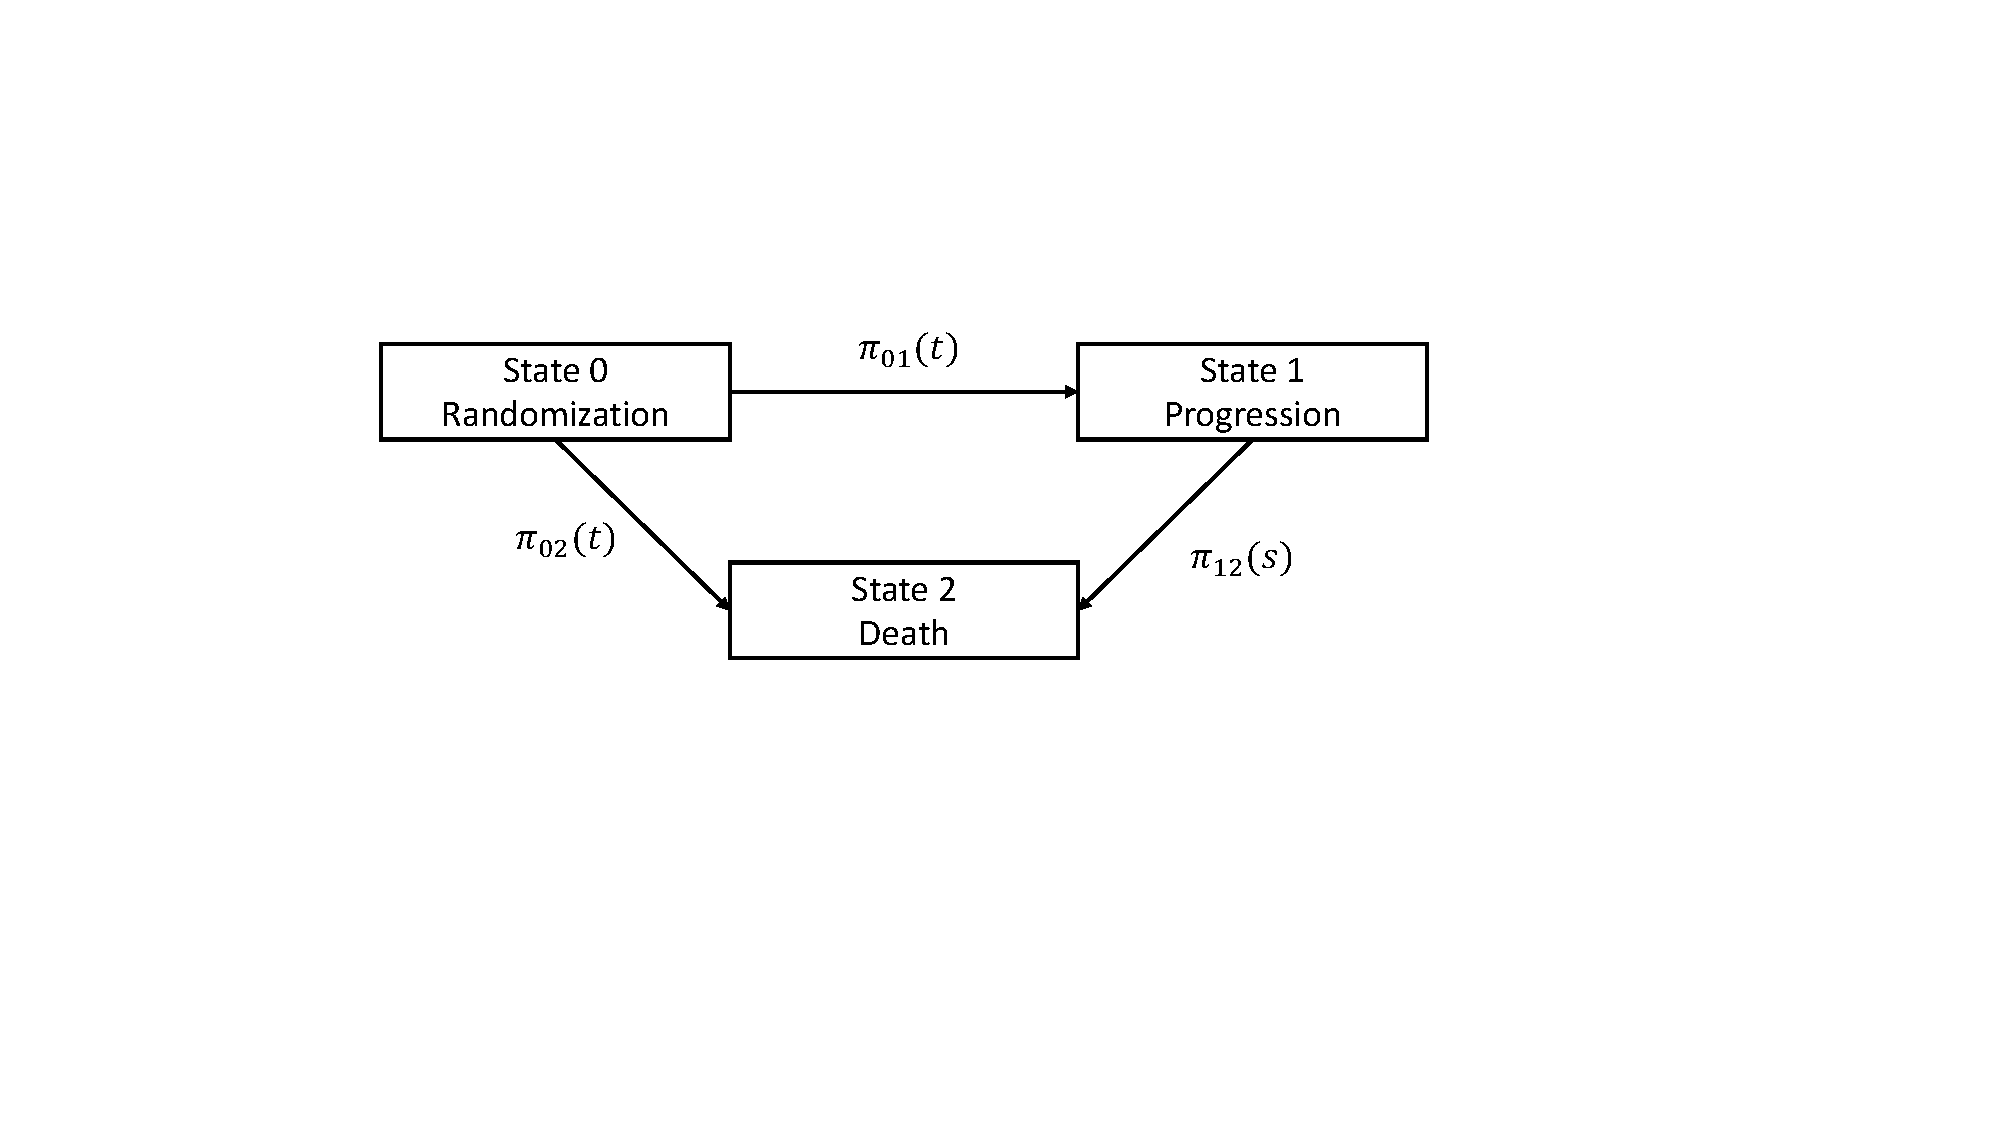
\includegraphics[width=0.8\textwidth]{img/multi-state.pdf}
    \caption{The multi-state (three-state illness-death) model \label{fig:multistate}}
\end{figure}

\newpage
\section{Likelihood derivation for the multi-state model}
For the multi-state model, we aim to estimate the parameter vector
\[
\theta = (\alpha, \gamma_{01}, \gamma_{02}, \gamma_{12})
\]
using maximum likelihood estimation.

\textbf{Modeling the Survival Experiences}:

Individual survival experiences can be characterized by four distinct cases based on a patient's progression through the multi-state model:

\begin{enumerate}
    \item Patients progress and are then censored.
    \item Patients progress and subsequently die.
    \item Patients die without prior progression.
    \item Patients are censored without experiencing either progression or death.
\end{enumerate}

For every individual \( i \) in the set \( (1, ..., n) \):

\begin{itemize}
    \item \( t_{i1} \) indicates the duration from the initial state to either progression or death.
    \item \( t_{i2} \), which is conditioned on progression, represents the time from progression to death.
\end{itemize}

\textbf{Likelihood Estimation for Individual Experiences}:

The individual likelihood for these experiences, denoted as \( L_i^{(k)}(\theta) \) where \( k \) varies from 1 to 4, can be described as:

\[
L_i^{(1)}(\theta) = f_1(t_{i1})S_2(t_{i1})S_3(t_{i2})
\]

\[
L_i^{(2)}(\theta) = f_1(t_{i1})S_2(t_{i1})f_3(t_{i2})
\]

\[
L_i^{(3)}(\theta) = S_1(t_{i1})f_2(t_{i1})
\]

\[
L_i^{(4)}(\theta) = S_1(t_{i1})S_2(t_{i1})
\]

Here:

\begin{itemize}
    \item \( f_1(\cdot) \) and \( S_1(\cdot) \): Density and survival function for time to progression.
    \item \( f_2(\cdot) \) and \( S_2(\cdot) \): Density and survival function for time to death without progression.
    \item \( f_3(\cdot) \) and \( S_3(\cdot) \): Density and survival function for time to death post progression.
\end{itemize}

\textbf{Overall Log-Likelihood}:

The comprehensive log-likelihood for all subjects can be formulated as:

\[
\begin{aligned}
\log(L(\theta)) &= \sum_{i=1}^{n}(d_1)(1-d_2)(1-d_3)L_i^{(1)}(\theta) \\
&\quad + (d_1)(1-d_2)(d_3)L_i^{(2)}(\theta) \\
&\quad +(1-d_1)(d_2)L_i^{(3)}(\theta) \\
&\quad +(1-d_1)(1-d_2)L_i^{(4)}(\theta),
\end{aligned}
\]

Where:

\begin{itemize}
    \item \( d_1 \): Indicator for progression.
    \item \( d_2 \): Indicator for death without preceding progression.
    \item \( d_3 \): Indicator for death post progression.
\end{itemize}

Note: An indicator value of 0 represents censoring, whereas a value of 1 indicates the event's occurrence.


\begin{table}
\caption{The coverage rate (CR) and credible interval (CI) width for predictors of the time of the last death. Comparing the results from the multivariate joint modeling approach (JM), a copula model between TTP and OS (Cop), a multi-state model (MS), and the marginal Weibull baseline hazard model of OS (Mrgl). The unit for CI width is month.  \label{tab:sim_result}}
\begin{center}
\begin{tabular}{ccccccccccccc}
& \multicolumn{4}{c}{Independent OS} & \multicolumn{4}{c}{OS dependent on NL} & \multicolumn{4}{c}{OS dependent on TL} \\ 
& JM & Cop & MS & Mrgl & JM & Cop & MS & Mrgl & JM & Cop & MS & Mrgl \\ \hline
\multicolumn{10}{l}{\textit{100 death event}}\\
CR & 0.49 & 0.49 & 0.01 & 0.00 & 0.11 & 0.11 & 0.03 & 0.00 &  0.91 & 0.91 & 1.00 & 0.00 \\ 
Width & 35.9 & 35.8 & 24.9 & 3.4  & 29.2 & 29.5 & 26.8 & 2.9  &  24.4 & 25.4 & 41.8 & 3.2 \\ \hline
\multicolumn{10}{l}{\textit{200 death event}}\\
CR & 0.89 & 0.86 & 0.33 & 0.00 & 0.45 & 0.45 & 0.24 & 0.00 & 0.85 & 0.98 & 1.00 & 0.00 \\ 
Width & 35.7 & 35.3 & 26.0 & 5.9 & 32.2 & 32.2 & 26.8 & 5.6 & 15.2 & 17.1 & 39.6 & 4.1  \\ \hline
\multicolumn{10}{l}{\textit{300 death event}}\\
CR & 0.98 & 0.98 & 0.98 & 0.00 & 0.90 & 0.89 &  0.95 & 0.01  & 0.97 & 0.98 & 1.00 & 0.00 \\ 
Width & 30.5 & 30.5 & 29.6 & 9.3 & 32.5 & 32.6 & 31.5 & 9.9 & 12.0 & 11.2 & 36.7 & 4.6 \\ 
\hline
\end{tabular}
\end{center}
\end{table}

\newpage
\begin{figure}[H]
\centering
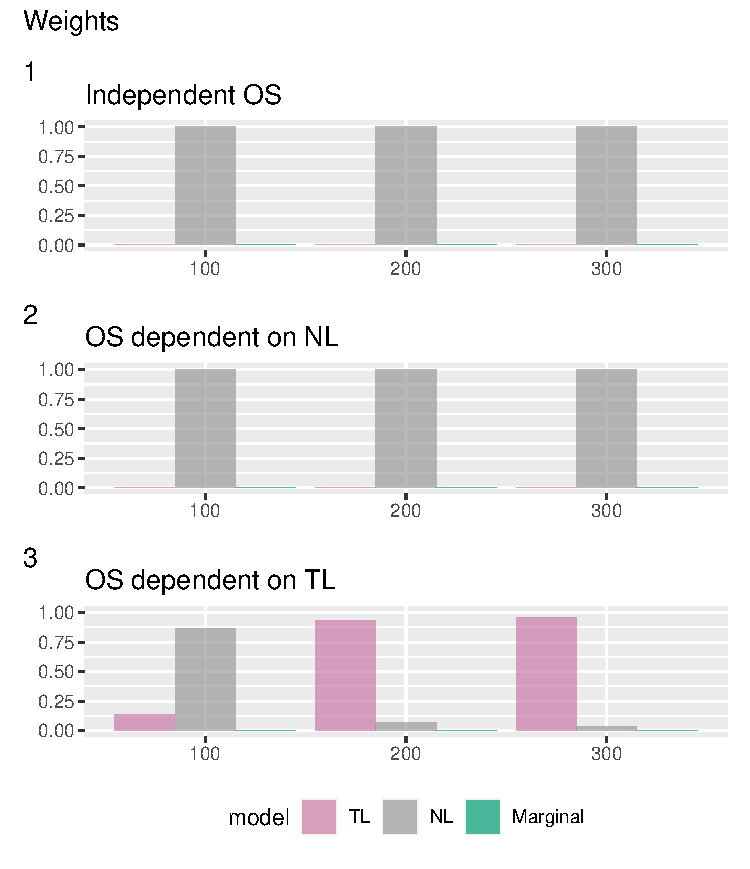
\includegraphics[width=0.7\textwidth]{img/Weights_simulation.pdf}
\caption{The weights of all submodels of the multivariate joint modeling approach for each snapshot dataset in the simulation studies.\label{fig:weights_simulation}}
\end{figure}

\newpage

\includepdf[pages=-,pagecommand=\thispagestyle{empty}]{diag.pdf}
%\bigskip
%\begin{center}
%{\large\bf SUPPLEMENTARY MATERIAL}
%\end{center}

%\begin{description}

%\item[Title:] Brief description. (file type)

%\item[R-package for  MYNEW routine:] R-package ÒMYNEWÓ containing code to perform the diagnostic methods described in the article. The package also contains all datasets used as examples in the article. (GNU zipped tar file)

%\item[HIV data set:] Data set used in the illustration of MYNEW method in Section~ 3.2. (.txt file)

%\end{description}

%\section{BibTeX}

%We hope you've chosen to use BibTeX!\ If you have, please feel free to use the package natbib with any bibliography style you're comfortable with. The .bst file agsm has been included here for your convenience. 

%\bibliographystyle{Chicago}

%\bibliography{Bibliography-MM-MC}
\end{document}
